\documentclass{report}
\usepackage[utf8]{inputenc}
\usepackage[T1]{fontenc}
\usepackage{circuitikz}
\usepackage{caption}
\usepackage{amsmath}
\usepackage{array}
\usepackage{pgfplots}
\usepackage{listings}
\usepackage{float}
\renewcommand{\figurename}{Slika}

\title{Projekat \\ \large{Osnovi digitalne elektronike}}

\author{Lazar Premović 0091/2019 \\ Anastasija Volčanovska 0092/2019 \\ Luka Simić 0368/2019}
\date{Maj 2021}

\begin{document}
    \maketitle
    \section*{Mikrokontroler}
        Program za mikrokontroler se sastoji iz četiri dela:
        \begin{itemize}
            \item Inicijalizacija registara, podataka i periferija
            \item Glavna petlja: Čitanje sa UART i postavljanje PWM registara
            \item Glavna petlja: Detekcija promene na A/D konvertoru i slanje na UART
            \item Prekidna rutina A/D konvertora
        \end{itemize}
        \subsection*{Inicijalizacija}
            U projektu rukovodimo sa četiri različita resursa: PWM, A/D konvertorom, UART i LCD monitorom, pa stoga moramo svakog od njih i da inicijalizujemo na početku izvršavanja programa.
            \subsubsection*{PWM}
                Za PWM deo,
                \begin{itemize}
                    \item postavljamo pinove porta D kao digitalne jer se pin RD1 koristi za PWM (CCP4),
                    \item postavljamo Capture and Compare modul 4 u PWM režim,
                    \item resetujemo registre za Duty Cycle Ratio,
                    \item postavimo frekvenciju na 80kHz na osnovu formule \eqref{PWMFreq} i
                    \item podesimo da se za PWM koristi Timer4 brojač koji zatim i uključimo.
                \end{itemize}
                Frekvencija PWM signala se u našem slučaju računa na osnovu sledeće jednačine sa strane 181 \textit{datasheet}-a za naš mikrokontroler:
                \begin{equation}
                    \label{PWMFreq}
                    F = \frac{1}{(PR_4 + 1) \cdot 4 \cdot T_{osc} \cdot Prescale_4}
                \end{equation}
                Vrednost $PR_4$ dobijamo izračunavajući gornju jednačinu:
                $$\frac{1}{80kHz} = (PR_4 + 1) \cdot 4 \cdot \frac{1}{8MHz} \cdot 1$$
                $$PR_4 = \frac{8MHz}{80kHz \cdot 4} - 1$$
                $$PR_4 = 24$$
            \subsubsection*{A/D konvertor}
                Za A/D konverziju,
                \begin{itemize}
                    \item biramo pin RA1 (kanal AN1) koji postavljamo kao analogni i ulazni,
                    \item referentni napon postavljamo na 5V, rezultat postavljamo da viši bitovi svi budu u višem registru,
                    \item vreme akvizicije i takt konverzije postavljamo po izboru,
                    \item palimo A/D konvertor i
                    \item podešavamo registre u vezi sa prekidima kako bismo dobijali prekid od A/D konvertora pri svakoj završenoj konverziji.
                \end{itemize}
            \subsubsection*{UART}
                Za komunikaciju preko UART,
                \begin{itemize}
                    \item postavljamo pinove porta C kao digitalne,
                    \item inicijalizujemo UART modul sa \textit{baud rate} od 9600,
                    \item čekamo određeno vreme da se UART komunikacija uspostavi i
                    \item podešavamo da čitamo prvi karakter ulaza.
                \end{itemize}
            \subsubsection*{LCD}
                LCD monitor inicijalizujemo i isključujemo mu prikazivanje kurzora. Pinovi porta B, gde je postavljen LCD monitor, su tom prilikom postavljeni kao digitalni. Takođe su inicijalizovane promenljive za čitanje vrednosti za A/D konvertora kao i šablonska niska koja se koristi pri ispisu pročitanog napona na LCD i UART.
        \subsection*{Čitanje sa UART}
            Prvi deo projekta nalaže da mikrokontroler treba da čita napon zadat sa PC računara i da postavlja da srednja vrednost PWM naponskog signala bude zadate vrednosti. Deo za čitanje je realizovan tako što se u glavnoj petlji proverava spremnost UART modula za čitanje, čita se jedan karakter, smešta se u nisku sa pročitanom porukom i kad se naiđe na karakter sa ASCII vrednošću 0 proverava se dužina poruke. Ukoliko je dužina poruke 5, to znači da je podatak uspešno primljen sa PC računara a zatim se iz nje iščitavaju vrednosti cifara i formira se broj koji predstavlja zadati napon.

            Kada imamo zadati srednji napon, treba da postavimo određene registre za PWM režim kako bismo dobili da taj napon bude srednja vrednost na pinu RD1. Kako se srednja vrednost napona računa na osnovu \textit{Duty Cycle Ratio} (DCR):
            $$V_{sr} = V_{ref} \cdot DCR$$
            a DCR kao:
            $$DCR = \frac{CCPR4L:CCP4CON_{5..4}}{4(PR_4 + 1)}$$
            dobijamo da nam dati registri moraju biti postavljeni na:
            $$CCPR4L:CCP4CON_{5..4} = DCR \cdot 100 = \frac{V_{sr}}{5} \cdot 100 = V_{sr} \cdot 20$$
            pa smo te vrednosti i upisali. Na kraju, resetujemo koji bajt poruke čitamo.
        \subsection*{Čitanje sa A/D konvertora}
            Čitanje sa A/D konvertora se realizuje iz dva dela. Prvi deo je prekidna rutina koja se poziva kada A/D konvertor završi konverziju, u kojoj se taj podatak učitava u promenljivu iz registara konvertora i ponovo pokreće A/D konvertor. Drugi deo je detekcija kada se vrednost na pinu promeni za više od 0.01V, u kom tu vrednost formatiramo u nisku, ispisujemo na LCD ekran, i istu nisku šaljemo preko UART PC računaru (karakter V se koristi kao oznaka za kraj poruke).
    \section*{PC}
        Program za PC je pisan na programskom jeziku C\# i sastoji se od dela za biranje i povezivanje na serijski port, dela za zadavanje napona koji odmah taj napon i šalje na serijski port i dela koji prikazuje pročitani napon sa A/D konvertora. Izgled interfejsa se može videti na slici \ref{GUI}.
        \begin{figure}[H]
            \centering
            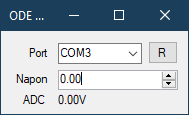
\includegraphics[scale=3]{GUI.png}
            \caption{Izgled grafičkog interfejsa programa za PC.}
            \label{GUI}
        \end{figure}
\end{document}
